\section{Scheduling}
\label{Scheduling}

\subsection{Multitasking}

Mehrere (gleiche oder unterschiedliche) Tasks müssen erledigt werden. Dazu werden Ressourcen benötigt (z.B. \textbf{CPU}, Speicher, ...).
Wenn mehrere Tasks \textbf{dieselben Ressourcen} benötigen, nimmt der \textbf{Scheduler} die Zuteilung der Ressourcen an die einzelnen Tasks vor.

\vspace{0.1cm}

Bei der Zuteilung der Ressourcen wird darauf geachtet, dass alle \textbf{kritischen deadlines eingehalten} werden. \\
\textrightarrow\ Der Scheduler \textbf{priorisiert} also die \textbf{kritischen Tasks.} \\
Unter Umständen werden somit Deadlines von weniger kritischen Tasks verletzt.


\subsubsection{Zeitdefinitionen (Task)}

\begin{center}
    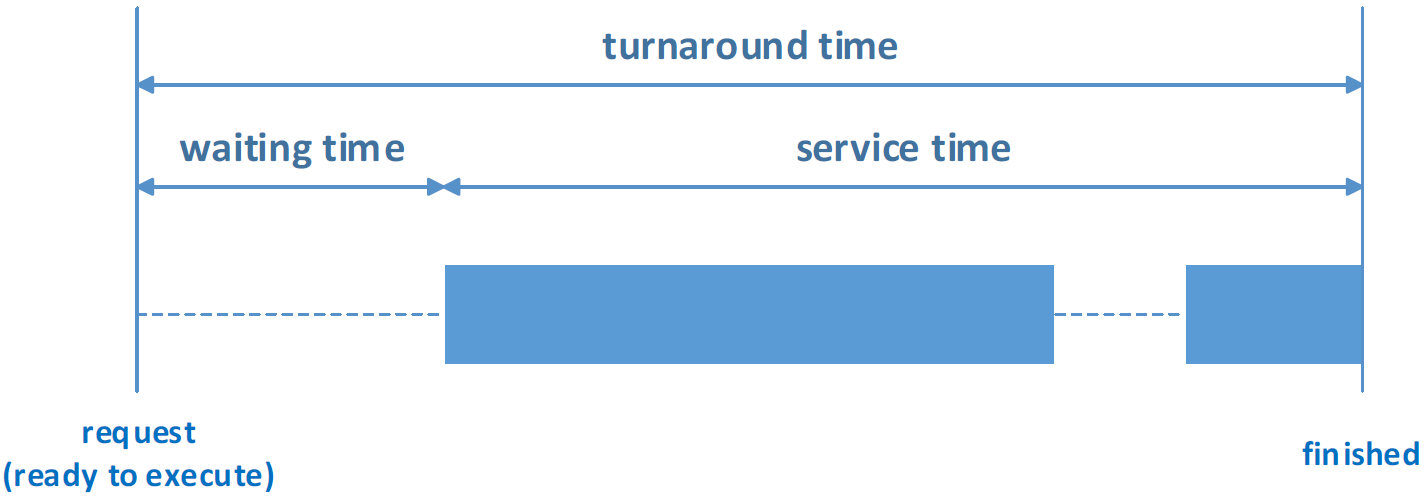
\includegraphics[width=0.8\columnwidth]{images/zeitdefinitionen_task.png}
\end{center}

\begin{outline}
    \1 \textbf{turnaround time:} (response time, Antwortzeit) 
        \2 Startet, wenn der Task bereit zur Ausführung ist und endet, wenn der Task fertig abgearbeitet ist
        \2 Zeit zwischen dem Vorhandensein von Eingangswerten an das System (Stimulus) bis zum Erscheinen der gewünschten Ausgangswerte.
    \1 \textbf{waiting time:} (Wartezeit)
        \2 Zeit zwischen Anliegen der Eingangswert und Beginn der Abarbeitung des Tasks
    \1 \textbf{service time:} (Bearbeitungszeit)
        \2 Zeit für Abarbeitung des Tasks \textrightarrow\ Unterbrechungen bzw. (preemptions) möglich 
\end{outline}


\subsubsection{Leistungsmerkmale}

\begin{minipage}[t]{0.52\columnwidth}
    \raggedright

    \begin{outline}
        \1 Durchsatz (throughput)
            \2 Anzahl erledigte Tasks pro Zeiteinheit
        \1 Mittlere Wartezeit (average waiting time)
    \end{outline}
\end{minipage}
\hfill
\begin{minipage}[t]{0.45\columnwidth}
    \raggedright

    \begin{outline}
        \1 Auslastung (utilization)
            \2 Prozentuale Auslastung einer Ressource
        \1 Weitere
    \end{outline}
\end{minipage}


\subsection{Scheduability}

Eine Menge von Tasks ist dann \textbf{scheduable}, wenn \textbf{alle Tasks zu allen Zeiten ihre deadlines einhalten} können. 
\textrightarrow\ Das ist immer das Ziel!

\subsubsection{Deadline -- Definition}

\begin{outline}
    \1 Spätestmöglicher Abschlusszeitpunkt (eines Tasks)
        \2 Bei periodischen Tasks ist dies meist gleichzeitig mit Beginn der nächsten Periode
\end{outline}


\subsection{Scheduling-Strategien}
\label{Scheduling-Strategien}

Folgende Algorithmen können für die Zuteilung der Ressourcen (Scheduling) verwendet werden:

\vspace{0.1cm}

\begin{minipage}[t]{0.46\columnwidth}
    \raggedright

    \begin{outline}
        \1 \textbf{FCFS (First Come First Served)}
            \2 Einfachste Variante
        \1 \textbf{Round Robin}
            \2 Rund herum in fixer Reihenfolge
        \1 \textbf{Random}
    \end{outline}
\end{minipage}
\hfill
\begin{minipage}[t]{0.5\columnwidth}
    \raggedright

    \begin{outline}
        \1 \textbf{SJF (Shortest Job First)}
            \2[+] Mittlere Wartezeit minimal
            \2[-] längere Tasks können 'verhungern'
        \1 \textbf{Priority Scheduling}
            \2 unterbrechbar (preemptive) oder nicht unterbrechbar (non-preemptive)
            \2[-] tief priorisierte Taks können 'verhungern'
    \end{outline}
\end{minipage}

\vspace{0.1cm}

\textbf{Hinweis:} 'verhungern' heisst, dass ein Task gar keine Ressourcen erhält


\subsection{Cooperative Multitasking}

Kooperative Task-Zuteilung ist bei \textbf{fairen} Tasks möglich.

\vspace{0.1cm}

\begin{outline}
    \1 Aktiver Task entscheidet selbst, wann er CPU wieder für andere Tasks freigibt
        \2 Unfaire und abgestürzte Tasks blockiert andere Tasks
    \1 Nächster Task kann mit beliebigem Algorithmus ermittelt werden \\
        \textrightarrow\ siehe Abschnitt \ref{Scheduling-Strategien}
    \1 Sehr einfach zu implementieren
\end{outline}


\subsection{Preemptive Multitasking / Scheduling}
\label{Preemptive Multitasking / Scheduling}

Preemptive Multitasking wird meistens in RTOS verwendet. \\
\textbf{Der Task mit höchster Priorität wird immer ausgeführt.} Unter Umständen muss dabei ein Task mit niedrigerer Priorität
\textbf{unterbrochen} werden. 

\vspace{0.1 cm}

Es gibt zwei Arten von Preemptive Multitasking Algorithmen:

\begin{outline}
    \1 \textbf{dynamic-priority Algorithmen}
        \2 Prioritäten werden zur Laufzeit laufen angepasst (z.B. aufgrund von vorhandenen deadlines)
    \1 \textbf{static-priority Algorithmen}
        \2 Prioritäten werden zur Entwicklungszeit festgelegt und nicht geändert.
        \2 Einfacher als dynamic-priority Algorithmen!
\end{outline}


\subsection{Rate Monotonic Scheduling (RMS)}

RMS beschreibt Regel, bei deren Einhaltung eine Konfiguration \textbf{immer scheduable} ist.


\subsection{Rate Monotonic Scheduling Theorem}
\label{Rate Monotonic Scheduling Theorem}

\subsubsection{Zwingende Voraussetungen}

\begin{itemize}
    \item Perioische Tasks
    \item static priority preemptive scheduling \textrightarrow\ siehe Abschnitt \ref{Preemptive Multitasking / Scheduling}
\end{itemize}


\subsubsection{Regeln für optimales Scheduling}

Für jeden Task $T_i$ wird die Periode $p_i$ und die (worst case) execution time $e_i$ ermittelt, bzw. geschätzt. \\
Die Prioritäten müssen den Tasks zwingend folgendermassen zugewiesen werden:

\vspace{0.1cm}

\textbf{Tasks mit kürzerer Periode (d.h. mit hoher Rate) erhalten höhere Priorität (rate-monotonic)}


\subsubsection{Berechnung der Auslastung einer Ressource}

\begin{minipage}[t]{0.48\columnwidth}
    Jeder Task $T_i$ trägt mit der Teilauslastung $u_i = \frac{e_i}{p_i}$ zur Gesamtauslastung $U$ bei.
\end{minipage}
\hfill
\begin{minipage}[t]{0.48\columnwidth}
    \vspace{-0.2cm}
    $$ U = \sum\limits_{i} \frac{e_i}{p_i} $$
\end{minipage}


\subsubsection{Auslastung einer Ressource}

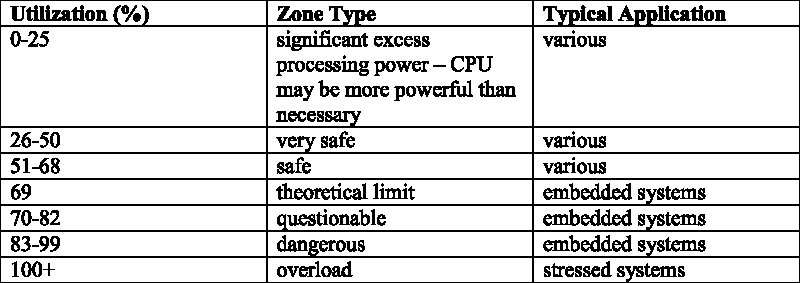
\includegraphics[width=\columnwidth]{images/tabelle_auslastung_system.pdf}


\subsection{Vorgehen -- Rate Monotonic Scheduling}

\begingroup
\renewcommand{\outlinei}{enumerate}
\renewcommand{\outlineii}{itemize}
\begin{outline}
    \1 Tasks priorisieren (Task mit kleinster Periode hat höchste Priorität!)
    \1 Task mit höchster Priorität aufzeichnen
    \1 Task mit zweithöchster Priorität 'regulär' zeichnen mit folgenden Sonderregelungen
        \2 Bei Bedarf warten (W), bis höher priorisierter Task abgeschlossen ist 
        \2 Höher priorisierte Tasks (bereits gezeichnet) unterbrechen (P) aktuellen Task
    \1 Punkt 3 wiederholen, bis alle Tasks aufgezeichnet sind und sich das Muster wiederholt
\end{outline}
\endgroup


\example{Rate Monotonic Scheduling}

\begin{minipage}[t]{0.55\columnwidth}
    Gemäss gegebener Tabelle sind die Tasks folgendermassen priorisiert:
    $$ T_1 > T_3 > T_2 $$
    In dieser Reihenfolge werden die Tasks aufgezeichnet!
\end{minipage}
\hfill
\begin{minipage}[t]{0.38\columnwidth}
    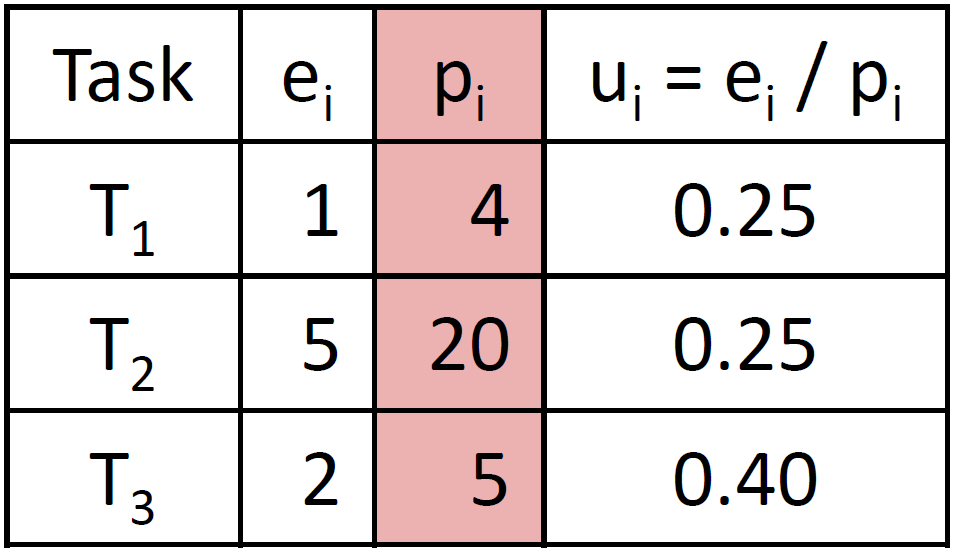
\includegraphics[width=\columnwidth, align=t]{images/scheduling_RMS_example_tabelle.png}
\end{minipage}

\begin{center}
    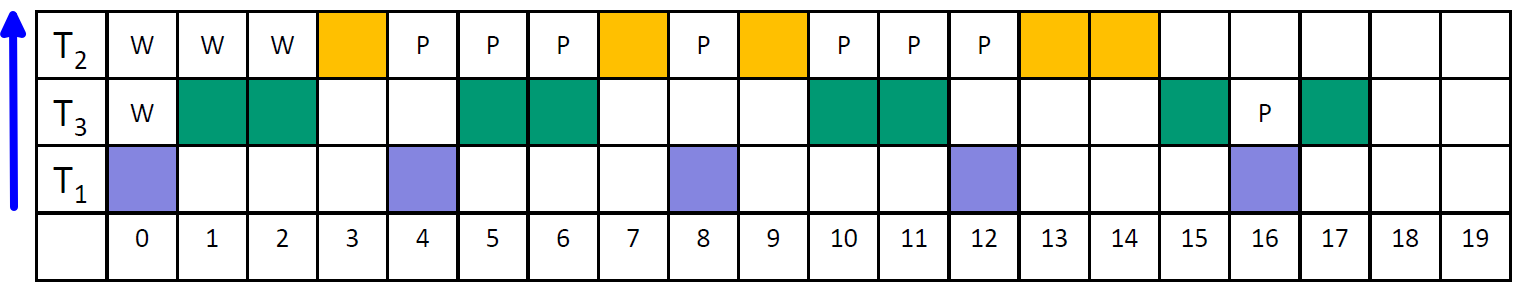
\includegraphics[width=\columnwidth]{images/scheduling_RMS_example_schedule.png}
\end{center}


\subsection{RMA Bound (RMA = Rate Monotonic Approach)}

Jede Konfiguration mit $n$ periodischen Tasks ist \textbf{immer} RM scheduable, wenn die Gesamtauslastung $U$ 
\textbf{unterhalb oder gleich} der RMA Bound $U(n)$ liegt

$$ \text{RMA-Bound} \qquad U(n) \leq n \cdot \big( 2^{\frac{1}{n}} - 1 \big)  $$

\begin{center}
    \begin{tabular}{l cccccc}
        \toprule
        $\bm{n}$                    & $2$       & $3$       & $4$       & $5$       & $10$      & $\infty$                      \\
        \midrule
        $\bm{U(n)}$ \textbf{in} \%  & $82.4$    & $78.0$    & $75.7$    & $74.4$    & $71.7$    & $\bm{\ln(2) \approx 69.3}$    \\
        \bottomrule
    \end{tabular}
\end{center}

\textrightarrow\ Liegt die Gesamtauslastung unter $69.3$ \%, ist die Konfiguration \textbf{immer} RM schedulable


\subsection{Anleitung für Zuweisung der Prioritäten bei RMS}

\begin{itemize}
    \item Prioritäten immer gemäss RMS zuweisen. (manuelle Zuweisung gibt keine bessere Lösung)
    \item Falls Auslastung nicht grösser als RMA Grenze, so ist Konfiguration RM schedulable
    \item Falls Auslastung \textbf{grösser} ist, muss \textbf{manuell analysiert} werden, ob Konfiguration schedulable ist
    \item 100 \% Auslastung könnte erreicht werden, wenn alle Perioden harmonisch sind, d.h. jede längere Periode ist ein exaktes
        Vielfaches aller Perioden kürzerer Dauer, \\
        z.B. (10, 20, 40, 80)
    \item Harmonische Perioden verringern die Unterbrechung (preemptions) von niedriger priorisierten Tasks \\
        \textrightarrow\ (10, 20, 40) ist gegenüber (10, 20, 50) zu bevorzugen, falls möglich
\end{itemize}

